\documentclass[aspectratio=169]{beamer}

\usetheme{Madrid}
\usecolortheme{seahorse}
\setbeamertemplate{navigation symbols}{}
\setbeamertemplate{footline}[frame number]

\usepackage{amsmath, amssymb}
\usepackage{listings}
\usepackage{xcolor}
\usepackage{tikz}
\usepackage{booktabs}
\usetikzlibrary{shapes.geometric, arrows.meta, positioning, patterns, decorations.pathreplacing}

% Code listing style
\lstdefinestyle{pysmall}{
  language=Python,
  basicstyle=\ttfamily\scriptsize,
  keywordstyle=\color{blue!80!black}\bfseries,
  commentstyle=\color{gray},
  stringstyle=\color{teal},
  backgroundcolor=\color{gray!8},
  frame=single,
  rulecolor=\color{gray!40},
  breaklines=true,
  showstringspaces=false,
}

\title[Local Mesh Refinement --- Poisson Solver]{%
  Local Mesh Refinement for the Poisson Equation\\
  \large Multi-Region Density Control in DOLFINx}
\author{Angel Ramirez}
\date{\today}

% ─────────────────────────────────────────────────────────────────────────────
\begin{document}

\begin{frame}
  \titlepage
\end{frame}

% ─────────────────────────────────────────────────────────────────────────────
\begin{frame}{Outline}
  \tableofcontents
\end{frame}

% ─────────────────────────────────────────────────────────────────────────────
\section{Motivation}

\begin{frame}{Why Local Refinement?}
  \begin{columns}
    \begin{column}{0.55\textwidth}
      \textbf{The problem with uniform meshes:}
      \begin{itemize}
        \item Physics varies wildly across the domain
        \item Near a gate or charge: fields change on nm scales
        \item Far from the source: nearly flat potential
        \item Uniform mesh wastes DOFs where nothing interesting happens
      \end{itemize}
      \vspace{0.8em}
      \textbf{The goal:}
      \begin{itemize}
        \item Fine mesh \emph{only} where needed
        \item Coarse mesh everywhere else
        \item Same accuracy, fraction of the runtime
      \end{itemize}
    \end{column}
    \begin{column}{0.42\textwidth}
      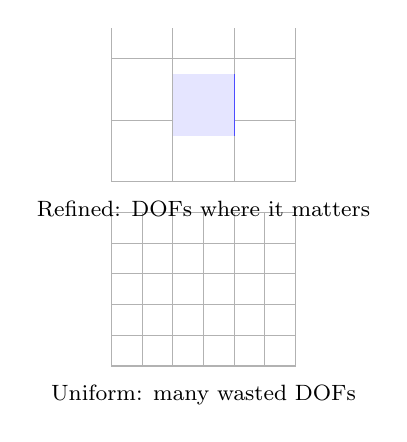
\begin{tikzpicture}[scale=0.78]
        % Uniform mesh cartoon
        \draw[gray!60, step=0.5] (0,0) grid (3,2.5);
        \node[below] at (1.5,-0.15) {\footnotesize Uniform: many wasted DOFs};

        % Locally refined cartoon
        \draw[gray!60, step=1.0] (0,3) grid (3,5.5);
        % fine inner
        \draw[blue!70, step=0.25] (1.0,3.75) grid (2.0,4.75);
        \fill[blue!10] (1.0,3.75) rectangle (2.0,4.75);
        \node[below] at (1.5,2.85) {\footnotesize Refined: DOFs where it matters};
      \end{tikzpicture}
    \end{column}
  \end{columns}
\end{frame}

% ─────────────────────────────────────────────────────────────────────────────
\begin{frame}{The Physical Problem}
  We solve the \textbf{Poisson equation} in a 3-D semiconductor/vacuum domain:
  \[
    -\nabla \cdot \bigl(\varepsilon \nabla \varphi\bigr) = \rho
  \]
  \begin{itemize}
    \item $\varphi$ — electrostatic potential
    \item $\varepsilon$ — permittivity (can be piecewise, e.g.\ Si/SiO$_2$)
    \item $\rho$ — free charge density (point charge, gate, etc.)
  \end{itemize}

  \vspace{0.6em}
  \textbf{Key lengthscales in a real device:}

  \begin{center}
  \begin{tabular}{lll}
    \toprule
    Region & Typical scale & Why it matters \\
    \midrule
    Gate / contact & $1$--$10$\,nm & Strong field gradient \\
    Semiconductor body & $50$--$200$\,nm & Moderate variation \\
    Far-field / contacts & $500$--$1000$\,nm & Nearly flat, cheap \\
    \bottomrule
  \end{tabular}
  \end{center}
\end{frame}

% ─────────────────────────────────────────────────────────────────────────────
\section{Implementation}

\begin{frame}{Architecture Overview}
  \begin{center}
  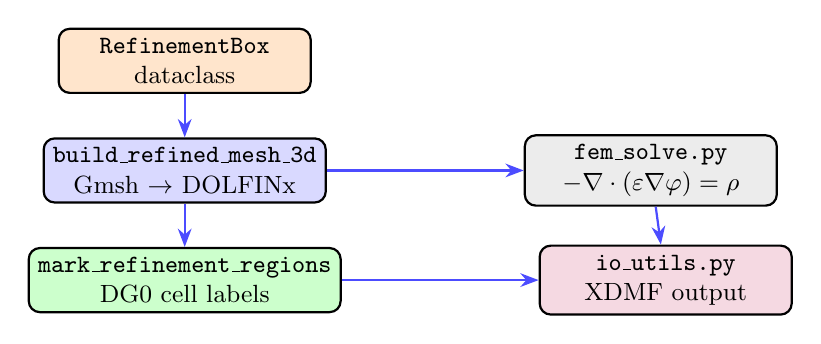
\begin{tikzpicture}[
      box/.style={rectangle, rounded corners=4pt, draw, thick,
                  minimum width=3.2cm, minimum height=0.8cm,
                  font=\small, align=center},
      arr/.style={-Stealth, thick, blue!70},
      node distance=0.55cm and 1.8cm
    ]
    \node[box, fill=orange!20] (rb) {\texttt{RefinementBox}\\dataclass};
    \node[box, fill=blue!15, below=of rb] (build) {\texttt{build\_refined\_mesh\_3d}\\Gmsh $\rightarrow$ DOLFINx};
    \node[box, fill=green!20, below=of build] (mark) {\texttt{mark\_refinement\_regions}\\DG0 cell labels};
    \node[box, fill=gray!15, right=2.5cm of build] (fem) {\texttt{fem\_solve.py}\\$-\nabla\cdot(\varepsilon\nabla\varphi)=\rho$};
    \node[box, fill=purple!15, right=2.5cm of mark] (io) {\texttt{io\_utils.py}\\XDMF output};

    \draw[arr] (rb) -- (build);
    \draw[arr] (build) -- (mark);
    \draw[arr] (build) -- (fem);
    \draw[arr] (fem)   -- (io);
    \draw[arr] (mark)  -- (io);
  \end{tikzpicture}
  \end{center}

  \vspace{0.4em}
  All new code lives in \texttt{src/poisson/refinement.py} and is exported
  at the package top-level.
\end{frame}

% ─────────────────────────────────────────────────────────────────────────────
\begin{frame}[fragile]{The \texttt{RefinementBox} Dataclass}
  A lightweight descriptor for one fine-mesh zone:

  \begin{lstlisting}[style=pysmall]
@dataclass
class RefinementBox:
    cx: float   # centre x (m)
    cy: float   # centre y (m)
    cz: float   # centre z (m)
    lx: float   # full width in x (m)
    ly: float   # full width in y (m)
    lz: float   # full width in z (m)
    h_fine: float  # target mesh size inside this box (m)
  \end{lstlisting}

  \vspace{0.5em}
  \textbf{Example — gate region:}
  \begin{lstlisting}[style=pysmall]
gate_box = RefinementBox(
    cx=0.0,  cy=0.0,  cz=15e-9,
    lx=80e-9, ly=80e-9, lz=30e-9,
    h_fine=4e-9,          # 4 nm mesh inside the gate area
)
  \end{lstlisting}
\end{frame}

% ─────────────────────────────────────────────────────────────────────────────
\begin{frame}[fragile]{Mesh Builder: Gmsh Box Fields}
  \texttt{build\_refined\_mesh\_3d} wraps the Gmsh API:

  \begin{enumerate}
    \item Create a single \texttt{occ.addBox} for the full domain
    \item For each \texttt{RefinementBox} add a Gmsh \textbf{Box field}
          (\texttt{VIn} = h\_fine, \texttt{VOut} = h\_coarse)
    \item Combine multiple fields with a Gmsh \textbf{Min field}\\
          $\Rightarrow$ finest rule wins everywhere
    \item Set as background mesh; disable size-from-points/curvature
    \item Convert to DOLFINx via \texttt{gmshio.model\_to\_mesh}
  \end{enumerate}

  \vspace{0.4em}
  \begin{lstlisting}[style=pysmall]
mesh = build_refined_mesh_3d(
    comm, Lx=500e-9, Ly=500e-9, Lz=150e-9,
    h_coarse=20e-9,
    boxes=[gate_box, interface_box],
)
  \end{lstlisting}
\end{frame}

% ─────────────────────────────────────────────────────────────────────────────
\begin{frame}{How the Min Field Works}
  \begin{center}
  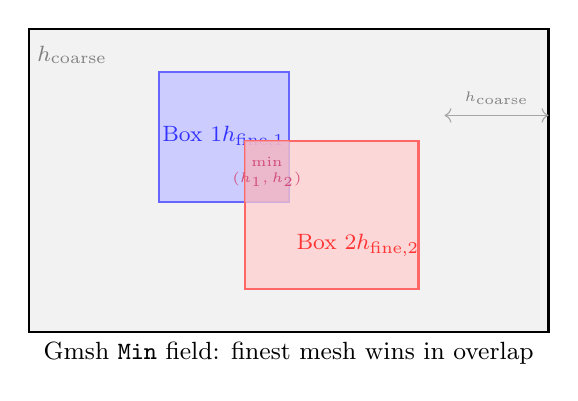
\begin{tikzpicture}[scale=1.1]
    % Domain
    \fill[gray!10] (0,0) rectangle (6,3.5);
    \draw[thick] (0,0) rectangle (6,3.5);
    \node[gray] at (0.5,3.2) {\footnotesize $h_\text{coarse}$};

    % Box 1
    \fill[blue!20] (1.5,1.5) rectangle (3.0,3.0);
    \draw[blue!60, thick] (1.5,1.5) rectangle (3.0,3.0);
    \node[blue!80, font=\footnotesize] at (2.25,2.25) {Box 1\\$h_\text{fine,1}$};

    % Box 2 (overlapping)
    \fill[red!20, opacity=0.7] (2.5,0.5) rectangle (4.5,2.2);
    \draw[red!60, thick] (2.5,0.5) rectangle (4.5,2.2);
    \node[red!80, font=\footnotesize] at (3.8,1.0) {Box 2\\$h_\text{fine,2}$};

    % Overlap label
    \fill[purple!30, opacity=0.7] (2.5,1.5) rectangle (3.0,2.2);
    \node[purple!70, font=\tiny, align=center] at (2.75, 1.85) {$\min$\\$(h_1,h_2)$};

    % h_coarse arrow
    \draw[<->, gray!70] (4.8,2.5) -- (6,2.5);
    \node[gray, font=\tiny] at (5.4, 2.7) {$h_\text{coarse}$};

    \node[below, font=\small] at (3,0) {Gmsh \texttt{Min} field: finest mesh wins in overlap};
  \end{tikzpicture}
  \end{center}
\end{frame}

% ─────────────────────────────────────────────────────────────────────────────
\begin{frame}[fragile]{Region Marker for Post-Processing}
  \texttt{mark\_refinement\_regions} labels each cell:

  \vspace{0.3em}
  \begin{center}
  \begin{tabular}{cl}
    \toprule
    DG0 value & Meaning \\
    \midrule
    0 & Coarse background \\
    1 & Inside \texttt{boxes[0]} \\
    2 & Inside \texttt{boxes[1]} \\
    $\vdots$ & $\vdots$ \\
    \bottomrule
  \end{tabular}
  \end{center}

  \vspace{0.5em}
  Uses cell midpoints (no DOLFINx locate overhead):
  \begin{lstlisting}[style=pysmall]
region = mark_refinement_regions(mesh, [gate_box, interface_box])
write_field_xdmf("out.xdmf", mesh, phi, region)
# In ParaView: color by 'refinement_region'
  \end{lstlisting}
\end{frame}

% ─────────────────────────────────────────────────────────────────────────────
\section{Point Charge Sweep}

\begin{frame}{Benchmark: Point Charge in Vacuum}
  \textbf{Problem:}
  \[
    -\nabla^2 \varphi = \rho_\sigma, \qquad
    \rho_\sigma = \frac{q}{(\sqrt{\pi}\,\sigma)^3}
    \exp\!\left(-\frac{r^2}{\sigma^2}\right)
  \]

  \begin{itemize}
    \item Gaussian-smoothed point charge, $\sigma = 3 h_\text{fine}$
    \item Exact Dirichlet BCs on all faces: $\varphi = \dfrac{q}{4\pi r}$
    \item Dimensionless: $q = 1$, $\varepsilon_0 = 1$
  \end{itemize}

  \vspace{0.5em}
  \textbf{Error metric:} mean relative error at 6 probe points at $r = L/3$:
  \[
    \bar{e}_\text{rel} = \frac{1}{N_p}\sum_i
      \frac{\lvert \varphi_h(\mathbf{x}_i) - \varphi_\text{ex}(r_i)\rvert}
           {\varphi_\text{ex}(r_i)}
  \]
\end{frame}

% ─────────────────────────────────────────────────────────────────────────────
\begin{frame}{10-Case Sweep Parameters}
  \begin{center}
  \renewcommand{\arraystretch}{1.25}
  \begin{tabular}{ccccl}
    \toprule
    Case & $L$ (nm) & $h_\text{fine}$ (nm) & $h_\text{coarse}$ (nm) & Regime \\
    \midrule
    1  &   20 &  1 &   4 & Tiny domain, ultra-fine \\
    2  &   50 &  1 &   8 & Small, very fine \\
    3  &  100 &  2 &  15 & Small \\
    4  &  200 &  2 &  20 & Medium-small \\
    5  &  200 &  4 &  40 & Medium-small, moderate \\
    6  &  300 &  4 &  60 & Medium \\
    7  &  500 &  4 &  80 & Medium-large \\
    8  &  500 &  8 & 160 & Medium-large, coarse \\
    9  &  800 &  8 & 160 & Large \\
    10 & 1000 & 10 & 320 & Very large, coarse \\
    \bottomrule
  \end{tabular}
  \end{center}

  \vspace{0.3em}
  Refinement box = $L/5 \times L/5 \times L/5$, centred at the charge.
  Run with \texttt{./scripts/run\_sweep.sh} from the repo root.
\end{frame}

% ─────────────────────────────────────────────────────────────────────────────
\begin{frame}{What the Sweep Reveals}
  \begin{columns}
    \begin{column}{0.48\textwidth}
      \textbf{Expected trends:}
      \begin{itemize}
        \item $\downarrow h_\text{fine}$ $\Rightarrow$ $\downarrow$ error,\\
              $\uparrow$ cells \& solve time
        \item $\uparrow h_\text{coarse}$ $\Rightarrow$ fewer far-field DOFs,\\
              but same near-field accuracy
        \item $\uparrow L$ $\Rightarrow$ BCs more accurate\\
              (charge looks more like a point)
      \end{itemize}
    \end{column}
    \begin{column}{0.48\textwidth}
      \textbf{CSV columns recorded:}
      \begin{itemize}
        \item \texttt{n\_cells}, \texttt{n\_dofs}
        \item \texttt{t\_mesh\_s} — Gmsh time
        \item \texttt{t\_solve\_s} — PETSc CG+AMG
        \item \texttt{t\_total\_s}
        \item \texttt{mean\_rel\_err}
      \end{itemize}
      \vspace{0.5em}
      \texttt{column -t -s, results/sweep.csv}
    \end{column}
  \end{columns}

  \vspace{0.6em}
  \begin{block}{Key insight}
    Fine mesh in a small refined box $+$ coarse mesh elsewhere
    $\approx$ same accuracy as uniform fine mesh
    at a \emph{fraction} of the DOF count and runtime.
  \end{block}
\end{frame}

% ─────────────────────────────────────────────────────────────────────────────
\section{Summary \& Next Steps}

\begin{frame}{Summary}
  \begin{enumerate}
    \setlength\itemsep{0.5em}
    \item \textbf{\texttt{RefinementBox}} — clean API to declare fine-mesh zones
          (centre, size, $h_\text{fine}$)
    \item \textbf{\texttt{build\_refined\_mesh\_3d}} — Gmsh-based builder, multiple
          boxes via Min field, outputs a DOLFINx mesh
    \item \textbf{\texttt{mark\_refinement\_regions}} — DG0 cell labels for
          diagnostics and material assignment
    \item \textbf{10-case sweep} — spans $L = 20$--$1000$\,nm,
          $h_\text{fine} = 1$--$10$\,nm, $h_\text{coarse} = 4$--$320$\,nm
    \item \textbf{Automatic timing + CSV} — mesh time vs.\ solve time,
          cell count, DOF count, relative error per case
  \end{enumerate}
\end{frame}

\begin{frame}{Next Steps}
  \begin{columns}
    \begin{column}{0.48\textwidth}
      \textbf{Physics extensions:}
      \begin{itemize}
        \item Multi-material $\varepsilon(x)$ with refinement at the interface
        \item Non-zero charge density $\rho$ with Neumann BCs for gates
        \item 2-D analogues using Gmsh \texttt{addRectangle} + Box field
      \end{itemize}
    \end{column}
    \begin{column}{0.48\textwidth}
      \textbf{Numerical extensions:}
      \begin{itemize}
        \item $h$-refinement convergence study (fix geometry, vary $h$)
        \item Compare uniform vs.\ locally refined at equal DOF count
        \item Extend to cylindrical / curvilinear refinement regions
        \item Adaptive refinement driven by residual error estimator
      \end{itemize}
    \end{column}
  \end{columns}
\end{frame}

% ─────────────────────────────────────────────────────────────────────────────
\begin{frame}{Repository Structure}
  \begin{center}
  \footnotesize
  \begin{tabular}{ll}
    \toprule
    File & Purpose \\
    \midrule
    \texttt{src/poisson/refinement.py}           & \textbf{New} — RefinementBox + mesh builder \\
    \texttt{src/poisson/fem\_solve.py}            & FEM assembly \& KSP solve \\
    \texttt{src/poisson/materials.py}             & Piecewise $\varepsilon$ (DG0) \\
    \texttt{src/poisson/io\_utils.py}             & XDMF write helpers \\
    \texttt{src/verify/local\_refinement\_demo.py}& \textbf{New} — 2-zone demo \\
    \texttt{src/verify/point\_charge\_sweep.py}   & \textbf{New} — sweep benchmark \\
    \texttt{scripts/run\_sweep.sh}                & \textbf{New} — 10-case runner \\
    \texttt{run\_dolfinx.sh}                      & Docker entry-point \\
    \bottomrule
  \end{tabular}
  \end{center}
\end{frame}

\end{document}
